\chapter{Weltflächen, Wick-Rotation und Kanald ualität}

\lectureoverview{Ein Teilchen beschreibt eine Weltlinie, eine Saite überstreicht eine Weltfläche. Die Quantisierung beider Objekte erfordert eine Summe über alle möglichen Verläufe, doch die lorentzsche Summe oszilliert und lässt sich nur schwer definieren. Ersetzt man die Weltflächenzeit durch eine imaginäre Koordinate, erhält man eine euklidische Theorie, die der Laplace-Gleichung gehorcht. Ihre konforme Symmetrie erlaubt es dann, die aufgeschlitzte Fläche einer Wechselwirkung mit vier Strings in eine Kreisscheibe mit vier Rand-Einsetzungen abzubilden. Dort wird die Symmetrie zwischen direktem und gekreuztem Kanal sichtbar.}

\section{Von der Weltlinie zur Summe über alle Verläufe}

Wir beginnen mit einem freien Teilchen. In der nichtrelativistischen Mechanik ist seine Position eine Funktion \(\mathbf x(t)\); bei auf eins gesetzter Masse lautet die Wirkung
\begin{equation}
  S_{\mathrm{NR}}[\mathbf x]
  =\frac12\int_{t_1}^{t_2}\dot{\mathbf x}^{\,2}\,dt.
  \label{eq:l07-nr-action}
\end{equation}
Für eine relativistische Beschreibung fasst man Raum und Zeit zweckmäßigerweise zu einem Vektor zusammen, \(X^\mu(\tau)\), der entlang der Bahn durch \(\tau\) parametrisiert wird. Der zugehörige quadratische Ausdruck lautet
\begin{equation}
  S_{\mathrm{rel}}[X]
  =\frac12\int_{\tau_1}^{\tau_2}
  \frac{dX^\mu}{d\tau}\frac{dX_\mu}{d\tau}\,d\tau.
  \label{eq:l07-rel-action}
\end{equation}
Die oberen und unteren Indizes kodieren den lorentzschen Vorzeichenunterschied zwischen Zeit und Raum.
\editorialnote{Die quadratische relativistische Wirkung wird hier für eine fest gewählte Parametrisierung der Weltlinie verwendet. Die manifest reparametrisierungsinvariante Alternative ist proportional zur Eigenlänge; sie wird später in der Vorlesung erwähnt.}

\begin{figure}[H]
  \centering
  \includegraphics[width=0.72\textwidth]{lecture_07_figure_01.png}
  \caption{Die nichtrelativistische Wirkung und ihr relativistisches quadratisches Gegenstück gemeinsam an der Tafel.}
  \lectureframe{00:03:35}
  \label{fig:l07-particle-actions}
\end{figure}

Klassisch fixiert man die Endpunkte und variiert den Weg. Ein freies Teilchen bewegt sich dann auf einer geraden Weltlinie mit konstanter Geschwindigkeit. Die Quantenmechanik stellt eine andere Frage. Sie wählt keine einzelne Bahn zwischen den Endpunkten aus, sondern fragt nach der Amplitude dafür, an einem Punkt zu starten und am anderen detektiert zu werden. Jeder dazwischenliegende Weg trägt eine Phase bei,
\begin{equation}
  K(2,1)=\int_{X(1)}^{X(2)}\!\mathcal D X\,
  e^{iS[X]}.
  \label{eq:l07-feynman-integral}
\end{equation}
Das Funktionalintegral ist ein Integral über einen unendlichdimensionalen Raum von Wegen und nicht das gewöhnliche Integral, das bereits in der Wirkung vorkommt.

\begin{figure}[H]
  \centering
  \includegraphics[width=0.72\textwidth]{lecture_07_figure_02.png}
  \caption{Ein beispielhafter Weg und die ihm zugeordnete Phase, bevor über alle Bahnen summiert wird.}
  \lectureframe{00:06:21}
  \label{fig:l07-path-integral-board}
\end{figure}

In der relativistischen Sprache ist diese Punkt-zu-Punkt-Amplitude ein Propagator. Bei einer Wechselwirkung treffen mehrere Weltliniensegmente zusammen. Man addiert ihre Wirkungen, integriert über die Treffpunkte und summiert über Diagramme mit den erforderlichen äußeren Teilchen. Die vertraute Entwicklung nach Feynman-Diagrammen ist somit bereits in der Anweisung enthalten, über alle Verläufe zu summieren.

Das Symbol \(S\) bezeichnet hier eine Wirkung. Es hat weder mit der Entropie noch mit der Mandelstam-Variablen \(s\) zu tun, die gegen Ende der Vorlesung verwendet wird. Die gemeinsame Notation ist traditionell, aber wenig aufschlussreich.

\section{Die Zeit imaginär werden lassen}

Mit \eqref{eq:l07-feynman-integral} tritt ein unmittelbares Problem auf. Jeder Faktor \(e^{iS}\) hat den Betrag eins. Eine stark oszillierende Bahn und die klassische gerade Linie gehen daher mit demselben absoluten Gewicht ein; sie unterscheiden sich nur in ihren Phasen. Durch destruktive Interferenz ergibt sich das klassische Verhalten, doch dadurch wird das formale Integral nicht zu einem gewöhnlichen konvergenten Objekt.

Führen wir einen neuen Parameter \(s\) ein, und zwar durch
\begin{equation}
  \tau=\alpha s,
  \qquad
  d\tau=\alpha\,ds,
  \qquad
  \frac{dX}{d\tau}=\frac{1}{\alpha}\frac{dX}{ds}.
\end{equation}
Dann skaliert die quadratische Wirkung wie folgt:
\begin{equation}
  \frac12\int d\tau
  \left(\frac{dX}{d\tau}\right)^2
  =
  \frac{1}{2\alpha}\int ds
  \left(\frac{dX}{ds}\right)^2.
  \label{eq:l07-rescaled-action}
\end{equation}
Die Wahl der Kontur entsprechend \(\alpha=-i\) verwandelt das oszillierende Gewicht in
\begin{equation}
  e^{iS}
  \longrightarrow
  \exp\!\left[-\frac12\int ds
  \left(\frac{dX}{ds}\right)^2\right]
  =e^{-S_E}.
  \label{eq:l07-euclidean-particle}
\end{equation}

\begin{figure}[H]
  \centering
  \includegraphics[width=0.66\textwidth]{lecture_07_figure_03.png}
  \caption{Das euklidische Teilchengewicht nach der Substitution der imaginären Zeit; der Exponent ist reell und nichtpositiv.}
  \lectureframe{00:16:20}
  \label{fig:l07-particle-wick}
\end{figure}

Eine Bahn, die weit hinaus- und wieder zurückläuft oder sich schnell hin und her windet, ohne dabei weit zu kommen, hat eine große positive \(S_E\) und wird daher exponentiell unterdrückt. Das Ergebnis ist ein Integral vom Wiener-Typ, für das eine fundierte Konvergenztheorie existiert. Die Endpunkte aus dem reellen \(\tau\) liegen auf einer imaginären Kontur in \(s\). In der Praxis wertet man das euklidische Objekt in seinem Konvergenzbereich aus und analytisch fortsetzt das Ergebnis anschließend zurück auf die physikalischen lorentzschen Variablen. Diese Operation ist die Wick-Rotation: Für die Rechnung wird die Zeit seitwärts gedreht, nicht verworfen.

\section{Von Weltlinien zu Weltflächen}

Ein Punktteilchen hat eine Weltlinie. Eine offene Saite überstreicht ein Band, eine geschlossene Saite einen Schlauch. Die Koordinaten \((\sigma,\tau)\) kennzeichnen Punkte auf dieser zweidimensionalen Weltfläche, während
\begin{equation}
  X^\mu=X^\mu(\sigma,\tau)
  \label{eq:l07-embedding}
\end{equation}
die Raumzeitposition des gekennzeichneten Punktes angibt. Kennt man alle Funktionen \(X^\mu\), so ist damit der vollständige Verlauf der Saite festgelegt.

Die quadratische lorentzsche Wirkung auf der Weltfläche hat dieselbe Struktur aus kinetischem und potentiellem Term mit entgegengesetzten Vorzeichen wie die Wirkung einer gewöhnlichen schwingenden Saite:
\begin{equation}
  S_{\mathrm{ws}}[X]
  =\frac{T_s}{2}\int d\tau\,d\sigma\,
  \left[
    \partial_\tau X^\mu\partial_\tau X_\mu
    -
    \partial_\sigma X^\mu\partial_\sigma X_\mu
  \right].
  \label{eq:l07-lorentzian-worldsheet}
\end{equation}
Die Gesamtspannung \(T_s\) legt die Skala fest; während sich die Vorlesung auf die Ableitungsstruktur konzentriert, wird sie unterdrückt.

\begin{figure}[H]
  \centering
  \includegraphics[width=0.72\textwidth]{lecture_07_figure_04.png}
  \caption{Die lorentzsche Wirkung auf der Weltfläche für
  \(X^\mu(\sigma,\tau)\), mit dem Vorzeichenunterschied zwischen kinetischem und potentiellem Term.}
  \lectureframe{00:24:26}
  \label{fig:l07-worldsheet-action}
\end{figure}

Die Stringamplitude erhält man, indem man diese Wirkung exponentiert und über alle Flächen summiert, die vorgegebene Anfangs- und Endkonfigurationen der Saite verbinden:
\begin{equation}
  \mathcal A=\int\mathcal D X\,e^{iS_{\mathrm{ws}}[X]}.
  \label{eq:l07-surface-integral}
\end{equation}
Dieselbe Vorschrift gilt für den Übergang von zwei Strings zu zwei, von zwei zu drei oder zu jeder anderen erlaubten äußeren Konfiguration. Auch verschiedene Topologien der Weltfläche gehen in die Summe ein. Das Hinzufügen von Löchern entspricht bei Strings dem Hinzufügen von Schleifenordnungen in der Diagrammentwicklung für Punktteilchen.

\begin{figure}[H]
  \centering
  \includegraphics[width=0.66\textwidth]{lecture_07_figure_05.png}
  \caption{Eine Fläche, die mehrere äußere Strings verbindet, mit einem Loch als Beispiel für eine andere Topologie der Weltfläche.}
  \lectureframe{00:27:14}
  \label{fig:l07-surface-topology}
\end{figure}

\begin{classroomqa}
\audiencequestion{Verschwindet bei einem Punkt-Elektron die Ableitung nach \(\sigma\) einfach? \lecturetimestamp{00:27:56}}
\lecturerresponse{Ein Punktteilchen hat von vornherein keine Koordinate \(\sigma\). Dennoch hängen die Bilder zusammen: Sind die äußeren Zustände im Vergleich zur Stringskala leicht und die Prozessenergien niedrig, reproduzieren Stringamplituden gewöhnliche Feynman-Diagramme für Punktteilchen. Dieser Grenzfall ergibt sich nicht einfach dadurch, dass man eine Ableitung auf null setzt.}
\end{classroomqa}

Das Flächenintegral hat dasselbe Konvergenzproblem wie das Pfadintegral. Nach der Wick-Rotation der Weltflächenzeit erhält man die stabile euklidische Form
\begin{equation}
  \begin{aligned}
    S_{E,\mathrm{ws}}[X]
    &=\frac{T_s}{2}\int d\tau\,d\sigma\,
      \left[
        \partial_\tau X^\mu\partial_\tau X_\mu
        +\partial_\sigma X^\mu\partial_\sigma X_\mu
      \right],\\
    \mathcal A_E&=\int\mathcal D X\,e^{-S_{E,\mathrm{ws}}}.
  \end{aligned}
  \label{eq:l07-euclidean-worldsheet}
\end{equation}
Nun treten beide Ableitungen mit demselben positiven Vorzeichen auf. Eine stark schwingende oder stark gedehnte Fläche hat eine große euklidische Wirkung und wird unterdrückt.

\begin{figure}[H]
  \centering
  \includegraphics[width=0.72\textwidth]{lecture_07_figure_06.png}
  \caption{Die positive euklidische Dichte auf der Weltfläche, nachdem \(\tau\) zur imaginären Zeit rotiert wurde.}
  \lectureframe{00:34:29}
  \label{fig:l07-worldsheet-wick}
\end{figure}

Es gibt auch eine geometrisch unmittelbarere Formulierung. Einem relativistischen Teilchen kann man eine Wirkung zuordnen, die proportional zur Eigenlänge seiner Bahn ist; einer Saite eine Wirkung proportional zur Raumzeitfläche ihrer Weltfläche. Letztere ist die Nambu--Goto-Wirkung. Die hier verwendete quadratische Form auf der Weltfläche wird üblicherweise als Polyakov-Form bezeichnet und ist für die vorliegende Rechnung wesentlich einfacher.
\editorialnote{Die Vorlesung enthält eine humorvolle Erörterung der historischen Namensgebung und erwähnt außerdem die verwandte Liouville-Wirkung sowie Dirichlet-Randbedingungen. Für die Herleitung ist keine Prioritätsbehauptung nötig; verwendet wird lediglich die Äquivalenz der Formulierungen mit Flächeninhalt und Hilfsmetrik.}

\section{Die euklidische Bewegungsgleichung}

Die Koordinaten \(\sigma\) und \(\tau\) sind lediglich Bezeichnungen auf der Fläche. Daher stellt sich unweigerlich die nächste Frage: Welche Umparametrisierungen lassen die Theorie unverändert? Am einfachsten lässt sich die Antwort anhand der Bewegungsgleichung erkennen. Die Variation von \eqref{eq:l07-euclidean-worldsheet} ergibt komponentenweise
\begin{equation}
  \partial_\tau^2X^\mu+\partial_\sigma^2X^\mu=0.
  \label{eq:l07-laplace}
\end{equation}
Vor der Wick-Rotation ist das relative Vorzeichen negativ; dann handelt es sich um eine Wellengleichung. Bei euklidischer Signatur sind beide Vorzeichen positiv, sodass sich die zweidimensionale Laplace-Gleichung ergibt.

\begin{classroomqa}
\audiencequestion{Ist das die Gleichung einer schwingenden Trommel?
\lecturetimestamp{00:41:50}}
\lecturerresponse{Sie ist eng damit verwandt, aber eine schwingende Trommel besitzt auch eine reelle Zeitkoordinate und gehorcht deshalb einer Wellengleichung. Die Gleichung hier ist die euklidische Laplace-Gleichung. Ein vertrauteres direktes Beispiel ist das elektrostatische Potential in einem ladungsfreien Gebiet.}
\end{classroomqa}

\begin{classroomqa}
\audiencequestion{Die Wirkung enthält erste Ableitungen. Warum enthält ihre Bewegungsgleichung dann zweite Ableitungen? \lecturetimestamp{00:42:44}}
\lecturerresponse{Bei der Variation eines Terms, der quadratisch in einer ersten Ableitung ist, und anschließender partieller Integration wird eine Ableitung auf diese erste Ableitung übertragen. Das ist die feldtheoretische Entsprechung dazu, dass in der Wirkung \(\dot x^{\,2}\) vorkommt und in der Bewegungsgleichung \(\ddot x\).}
\end{classroomqa}

\begin{figure}[H]
  \centering
  \includegraphics[width=0.68\textwidth]{lecture_07_figure_07.png}
  \caption{Die Laplace-Gleichung mit Pluszeichen und die erste diskrete Zeile zur Deutung ihrer zweiten Ableitungen.}
  \lectureframe{00:43:30}
  \label{fig:l07-laplace-board}
\end{figure}

Um die Geometrie zu erkennen, diskretisieren wir zunächst eine Koordinate mit dem Abstand \(\epsilon\). Eine erste Ableitung entspricht einer Differenz benachbarter Werte, eine zweite Ableitung der Differenz benachbarter Differenzen:
\begin{equation}
  \frac{d^2X}{ds^2}\bigg|_{2}
  \longrightarrow
  \frac{X(3)-2X(2)+X(1)}{\epsilon^2}.
  \label{eq:l07-second-difference}
\end{equation}

\begin{figure}[H]
  \centering
  \includegraphics[width=0.72\textwidth]{lecture_07_figure_08.png}
  \caption{Die nummerierte Zeile, ein kleines Gitterstück und die Differenzenentwicklung einer zweiten Ableitung.}
  \lectureframe{00:45:51}
  \label{fig:l07-finite-difference-board}
\end{figure}

Nun diskretisieren wir die \((\sigma,\tau)\)-Ebene. Die vier nächsten Nachbarn eines zentralen Punktes \(5\) bezeichnen wir mit \(1,2,3,4\). Gleichung \eqref{eq:l07-laplace} wird zu
\begin{equation}
  X(1)+X(2)+X(3)+X(4)-4X(5)=0,
\end{equation}
oder
\begin{equation}
  X(5)=\frac14\bigl[X(1)+X(2)+X(3)+X(4)\bigr].
  \label{eq:l07-mean-value}
\end{equation}

\begin{figure}[H]
  \centering
  \includegraphics[width=0.72\textwidth]{lecture_07_figure_09.png}
  \caption{Die vollständige zweidimensionale Differenzengleichung: Der Wert im Zentrum ist gleich dem Mittelwert seiner vier Nachbarwerte.}
  \lectureframe{00:48:26}
  \label{fig:l07-mean-value-board}
\end{figure}

Diese Mittelwerteigenschaft gilt für ein infinitesimales Quadrat beliebiger Orientierung. Sie ist der lokale geometrische Gehalt der Laplace-Gleichung und führt zur konformen Symmetrie.

\section{Konforme Koordinaten}

Betrachten wir eine Koordinatentransformation von \((\sigma,\tau)\) nach \((\sigma',\tau')\). Eine allgemeine Verformung bildet ein kleines Quadrat auf ein beliebiges Viereck ab. Die hier relevanten speziellen Transformationen bilden jedes infinitesimale Quadrat auf ein anderes infinitesimales Quadrat ab, das gedreht und skaliert sein kann. Äquivalent dazu bleibt der Winkel erhalten, unter dem sich Kurven schneiden. Solche Transformationen heißen konform.

\begin{figure}[H]
  \centering
  \includegraphics[width=0.68\textwidth]{lecture_07_figure_10.png}
  \caption{Ein kleines Quadrat wird lokal auf eine andere kleine Figur abgebildet; dabei wird geprüft, ob ihre Winkel unter der konformen Abbildung erhalten bleiben.}
  \lectureframe{00:53:25}
  \label{fig:l07-conformal-board}
\end{figure}

\begin{classroomqa}
\audiencequestion{Wenn die Winkel erhalten bleiben, ist die Transformation dann im Wesentlichen nur eine Drehung? \lecturetimestamp{00:53:31}}
\lecturerresponse{Nur lokal, und selbst dort ist auch eine gemeinsame Skalierung erlaubt. Der lokale Drehwinkel und der Skalierungsfaktor können sich von Punkt zu Punkt ändern. So kann sich das Koordinatengitter krümmen, sich in einem Bereich ausdehnen und in einem anderen zusammenziehen, während infinitesimale Formen erhalten bleiben.}
\end{classroomqa}

Eine winkelbewahrende Abbildung muss nicht die Größe erhalten. Würde auch die Größe überall festgehalten, bliebe nur die wesentlich kleinere Klasse starrer Transformationen aus Verschiebungen und Drehungen. Konforme Abbildungen erhalten stattdessen die lokale Form. Deshalb kann eine Kartenprojektion die Form einer kleinen Insel bewahren, während sie deren Fläche stark verzerrt.

\begin{classroomqa}
\audiencequestion{Bedeutet konforme Abbildung dasselbe wie ein flaches Koordinatensystem? \lecturetimestamp{00:55:35}}
\lecturerresponse{Nein. Flachheit und Konformität sind unterschiedliche Aussagen. Eine konforme Abbildung kann gekrümmte Koordinatenlinien verwenden; erhalten bleibt der Winkel zwischen sich schneidenden Kurven. Eine Projektion vom Mercator-Typ ist ein vertrautes Beispiel: Sie bewahrt die lokale Form, verzerrt aber die Skala erheblich.}
\end{classroomqa}

In zwei Dimensionen werden die benötigten Transformationen lokal durch analytische Funktionen einer komplexen Koordinate erzeugt:
\begin{equation}
  z=\sigma+i\tau.
\end{equation}
Endliche Gebiete können dabei sehr unterschiedlich aussehen. Ein quadratisches Gebiet kann auf ein glattes Gebiet abgebildet werden, wobei die ursprünglichen Ecken auf gewöhnliche Randpunkte statt auf die optisch auffälligen Punkte des neuen Randes abgebildet werden. Das ist kein Widerspruch: Konformität ist eine lokale Bedingung im Inneren, und die Abbildung erhält infinitesimale Winkel, sofern sie regulär ist.

\begin{classroomqa}
\audiencequestion{Ist diese Koordinatenfreiheit der Grund dafür, dass sich das frühere Diagramm mit dem Zusammenfügen--und Aufspalten symmetrisch wählen ließ?
\lecturetimestamp{00:56:32}}
\lecturerresponse{Ja. Dieselbe konforme Freiheit, die die Gleichungen auf der Weltfläche erhält, erlaubt es uns, den unhandlichen Wechselwirkungsstreifen durch einen symmetrischeren Bereich zu ersetzen. Die verbleibende Freiheit beseitigt den physikalischen Parameter für das Zusammenfügen--und Aufspalten nicht, sondern stellt ihn als relative Position der Rand-Einsetzungen dar.}
\end{classroomqa}

\section{Der aufgeschlitzte Streifen und die Kreisscheibe}

Kehren wir zur Streuung von vier Strings zurück. Zwei offene Strings treten ein, ihre Endpunkte verbinden sich, der zusammengesetzte String breitet sich aus und spaltet sich später wieder auf. Als flache Weltfläche gezeichnet, ist der Vorgang ein unendlicher Streifen, der von beiden Enden aus aufgeschlitzt ist. Der Abstand \(\tau_0\) zwischen den Spitzen der Schlitze entspricht der Lebensdauer des Zwischenzustands des Strings; über diesen Abstand wird in der Amplitude integriert.

\begin{figure}[H]
  \centering
  \includegraphics[width=0.72\textwidth]{lecture_07_figure_11.png}
  \caption{Der beidseitig aufgeschlitzte Streifen stellt dar, wie sich zwei offene Strings verbinden, gemeinsam ausbreiten und wieder aufspalten.}
  \lectureframe{01:00:20}
  \label{fig:l07-slit-strip}
\end{figure}

Nach der Euklidisierung gehorchen die Einbettungsfelder in diesem Gebiet der Laplace-Gleichung. Die konforme Invarianz erlaubt deshalb, den aufgeschlitzten Streifen auf eine Kreisscheibe abzubilden. Die Topologie lässt sich veranschaulichen, indem man die Kreisscheibe mit konzentrischen Kreisen foliierte und diese geschlossenen Kurven kontinuierlich verformt, bis sie das aufgeschlitzte Gebiet ausfüllen. Die Enden im Unendlichen werden unter der Abbildung zu ausgezeichneten Randpunkten.

\begin{figure}[H]
  \centering
  \includegraphics[width=0.72\textwidth]{lecture_07_figure_12.png}
  \medskip

  \begin{adjustbox}{max width=\linewidth}
  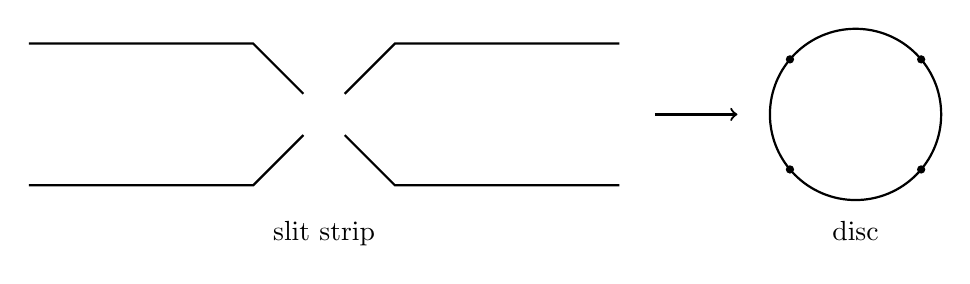
\begin{tikzpicture}[x=0.75cm,y=0.75cm]
    \draw[thick] (-5,1.2) -- (-1.2,1.2) -- (-0.35,0.35);
    \draw[thick] (-5,-1.2) -- (-1.2,-1.2) -- (-0.35,-0.35);
    \draw[thick] (0.35,0.35) -- (1.2,1.2) -- (5,1.2);
    \draw[thick] (0.35,-0.35) -- (1.2,-1.2) -- (5,-1.2);
    \draw[->,thick] (5.6,0) -- (7.0,0);
    \draw[thick] (9.0,0) circle (1.45);
    \foreach \a in {40,140,220,320} \fill (9.0,0) ++(\a:1.45) circle (1.5pt);
    \node[below] at (0,-1.65) {slit strip};
    \node[below] at (9.0,-1.65) {disc};
  \end{tikzpicture}
  \end{adjustbox}
  \caption{Vergleich der Niveaukurven an der Tafel und ein übersichtliches Schema der konformen Abbildung vom aufgeschlitzten Streifen auf eine Kreisscheibe. Die vier äußeren Enden werden zu vier ausgezeichneten Randpunkten.}
  \lectureframe{01:04:46}
  \label{fig:l07-strip-to-disc}
\end{figure}

Bei dieser Koordinatentransformation gehen die äußeren Zustände nicht verloren. An den vier ausgezeichneten Punkten müssen Impuls, Teilchentyp und Oszillatorniveau eingesetzt werden. Die formalen Objekte, die diese Informationen tragen, sind Vertexoperatoren. Ihre genaue Konstruktion wird zurückgestellt, doch ihre Rolle ist bereits klar: Sie machen aus einem ansonsten homogenen Pfadintegral auf der Weltfläche ein festgelegtes Streuexperiment.

Nachdem man mithilfe konformer Transformationen der Kreisscheibe drei Randpunkte auf zweckmäßige Referenzpositionen verschoben hat, bleibt eine reelle relative Position übrig. Sie lässt sich durch das Doppelverhältnis der vier geordneten Randpunkte darstellen. Auf der Kreisscheibe entspricht dies der früheren Lebensdauer \(\tau_0\).

\begin{figure}[H]
  \centering
  \includegraphics[width=0.62\textwidth]{lecture_07_figure_13.png}
  \caption{Vier Einsetzungspunkte am Rand der Kreisscheibe. Die konforme Freiheit lässt von ihrer geordneten Anordnung nur einen reellen Modul übrig.}
  \lectureframe{01:10:55}
  \label{fig:l07-four-points}
\end{figure}

Das Integral über die Lebensdauer ist also nicht verschwunden. Es ist zu einem Integral über den verbleibenden Modul geworden. Mit der üblichen Koordinate \(0<z<1\) hat das Vierpunktintegral für offene Strings dieselbe Form wie in der vorherigen Vorlesung:
\begin{equation}
  \mathcal A(s,t)\propto
  \int_0^1 z^{-s-1}(1-z)^{-t-1}\,dz.
  \label{eq:l07-modulus-integral}
\end{equation}

\section{Zwei Grenzfälle derselben Fläche}

An einem Ende des Modulraums rücken die beiden Einsetzungspunkte des einlaufenden Paares zusammen. In den Koordinaten des aufgeschlitzten Streifens entspricht dies einem langen Zeitintervall zwischen dem Zusammenfügen und dem Aufspalten: Ein Zwischenzustand des Strings im direkten Kanal breitet sich lange aus. Am anderen Ende rückt ein anderes benachbartes Paar zusammen. Dann lässt sich dieselbe Fläche auf natürliche Weise als Austausch im gekreuzten Kanal lesen. Auf dem Streifen wirken diese Beschreibungen unzusammenhängend, doch sie entsprechen benachbarten Randgrenzfällen desselben Integrals über die Kreisscheibe.

Kehren wir zur Mostly-Plus-Konvention der vorherigen Vorlesung zurück:
\begin{equation}
  -s=(k_1+k_2)^2,
  \qquad
  -t=(k_1+k_3)^2.
  \label{eq:l07-mandelstam}
\end{equation}
Der direkte Grenzfall ordnet die Pole in \(s\); der gekreuzte Grenzfall ordnet die Pole in \(t\).
\editorialnote{Gegen Ende der Vorlesung verwendet die Tafel eine abkürzende Vorzeichenkonvention für die Mandelstam-Variablen und setzt zugleich \(s\) mit dem positiven Quadrat der Schwerpunktsenergie gleich. In Gleichung \eqref{eq:l07-mandelstam} gilt die in Vorlesung 6 eingeführte Mostly-Plus-Konvention.}

\begin{figure}[H]
  \centering
  \includegraphics[width=0.62\textwidth]{lecture_07_figure_14.png}
  \caption{Die beiden Kanäle: lange Ausbreitung in der einen Orientierung und Austausch in der gekreuzten Orientierung.}
  \lectureframe{01:19:27}
  \label{fig:l07-channel-diagrams}
\end{figure}

\begin{figure}[H]
  \centering
  \includegraphics[width=0.72\textwidth]{lecture_07_figure_15.png}
  \caption{Die Tafel zeigt erneut die Impulszuordnungen im \(s\)- und \(t\)-Kanal und vergleicht dabei die beiden Grenzfälle des Moduls der Kreisscheibe.}
  \lectureframe{01:19:40}
  \label{fig:l07-st-board}
\end{figure}

Ein und dasselbe analytische Objekt liefert somit beide Entwicklungen:
\begin{equation}
  \mathcal A(s,t)=\mathcal A(t,s).
\end{equation}
Das ist die Kanald ualität. In der ursprünglichen Resonanzsprache wirkte es wunderbar, dass eine Summe über Zustände des direkten Kanals zugleich den Austausch im gekreuzten Kanal kodieren kann. Auf der euklidischen Weltfläche erklärt die konforme Symmetrie, warum beide Beschreibungen zu derselben Fläche gehören. Historisch folgte diese Deutung kurz nach der Entdeckung der Veneziano-Amplitude im Jahr 1969.

\begin{classroomqa}
\audiencequestion{Gibt es auch ein Bild des aufgeschlitzten Streifens für die gekreuzte Orientierung? \lecturetimestamp{01:20:49}}
\lecturerresponse{Ja, dafür muss man die Richtung, die man Zeit nennt, anders wählen. Dieselbe euklidische Fläche lässt sich so schneiden, dass ein anderes Paar äußerer Enden in ferner Vergangenheit und Zukunft liegt. Gerade diese alternative Schnittwahl erklärt, warum eine einzige Weltfläche mehr als eine Kanalinterpretation zulässt.}
\end{classroomqa}

\begin{classroomqa}
\audiencequestion{Wird die Zeit, während der die Strings verbunden bleiben, durch die Kopplungskonstante bestimmt? \lecturetimestamp{01:21:39}}
\lecturerresponse{Es wird keine feste Lebensdauer ausgewählt. Die Lebensdauer ist eine Integrationsvariable, und jeder Wert trägt bei. Die Kopplung bestimmt das Gewicht für das Zusammenfügen und Aufspalten---, gleichbedeutend mit der Zerfallsstärke---, und geht multiplikativ in die Amplitude ein; sie ersetzt nicht das Integral über den Modul.}
\end{classroomqa}
